\documentclass{article}

\usepackage[nonatbib, final]{dl}
%NOTE: to compile a camera-ready version, add the [final] option, e.g.:
\documentclass{article}
\usepackage[utf8]{inputenc}
\usepackage{graphicx}
\usepackage[colorlinks,linkcolor=red]{hyperref}
\usepackage{amsmath}
\usepackage[utf8]{inputenc}
\usepackage[T1]{fontenc}
\usepackage[pdftex,colorlinks]{hyperref}
\usepackage{url}
\usepackage{booktabs}
\usepackage{amsfonts}
\usepackage{nicefrac}
\usepackage{microtype}
\usepackage{threeparttable}

\title{A Solution to China Competitive Poker Using Deep Learning with Computer Generated Training Examples}

\author{
  Guo Luning \\
  The Chinese University of Hong Kong, Shenzhen\\
  \texttt{220041063@link.cuhk.edu.cn} \\
  %% examples of more authors
   \And
   Fang Zehao \\
   The Chinese University of Hong Kong, Shenzhen\\
   \texttt{220019098@link.cuhk.edu.cn} \\
   \And
   Qu Xiaodong \\
   The Chinese University of Hong Kong, Shenzhen\\
   \texttt{220019089@link.cuhk.edu.cn} \\
}

\def\PaperID{0035} % *** Enter your assigned Paper ID here

\begin{document}
\maketitle

\begin{abstract}
  In recent years, more and more people are interested in China Compatitive Poker (CCP), which we also call Doudizhu. There are many Doudizhu game platforms, and most of these platforms have a Doudizhu AI. However, none of these AIs is satisfactory, and they tend to have a very low winning rate when confronting real people. So, we want to train a new Doudizhu AI by using deep neural network, and we hope this AI will perform well against high-level players. As Doudizhu is a game of imperfect information (with private information, random) with multiple rounds of cooperation and competition, this causes us to have a varity of card strategies. In this project we introduce an approach to play Doudizhu by using Logistic Regression to predict if we bid or not, then we use  Convolutional Neural Network (CNN) to predict actions. This network is trained by supervised learning from our generated game records. This game records are generated by Minimax algorithm. And the final result is not bad compared to random algorithm.
\end{abstract}

\section{Introduction}

China Competitive Poker (CCP) is a poker game that vary famous in China. CCP is played among three people with one pack of cards, including two jokers. After bid, one player become the ``Landlord (or Declarer)'', the other players as``Peasant (or Defenders)'', they are a team competing against the ``Landlord''. It is a game that easy to learn but hard to master, requiring the mathematical and strategic thinking as well as carefully planned execution. In 2018, Tencent online game platform reported 30 million players attending annual Doudizhu championship. Although there are many AI robots that can play with people in different game platforms, we find that most of these AI get a very low winning rate when playing with human player.

Compared to other game such as Go, Doudizhu is a kind of imperfect information game, starts from a random state. A player gets different cards each game, does not know the cards distribution of the other two players. Like bridge, ``Peasants'' must coordinate with each other, otherwise they could hardly beat the ``Landlord''. Doudizhu is a good problem for game AI. In this project, we choose CNN to solve the problem in Doudizhu for the following reasons: First, there are little Doudizhu algorithms using CNN yet, we want to prove CNN can have good result compared to random strategy. Second, CNN has achieved superhuman performance in perfect information games, we want to see how CNN perform in inperfect information games. Third, there is semi-translational invariance in Doudizhu, e.g. there are two sets of cards in the same category but with different ranks (like ``34567'' and ``45678''), if we add each card's rank, then ``34567'' become ``45678'', this is translational invariance. The player can play out ``45678'' after another one played out ``34567'', but it is illegal if we swap the order, this is the reason for ``simi''.

In this paper, we proposed a new AI model structure. First we deal randomly, then we use Logestic Regression to determine whether to bid. After bid, we use CNN to train the player's strategy. The import of the policy net is related to the cards that the other player played. And we also designed a ``Kicker Net'' to determine which card to be taken. The entire game flow shows in Figure \ref{gameflow}. For the CNN model, we will give more detail information in Section 2.
\graphicspath{{Images/}}
\maketitle
\begin{figure}[htp]
    \caption{Game Flow} \label{gameflow}
    \centering 
    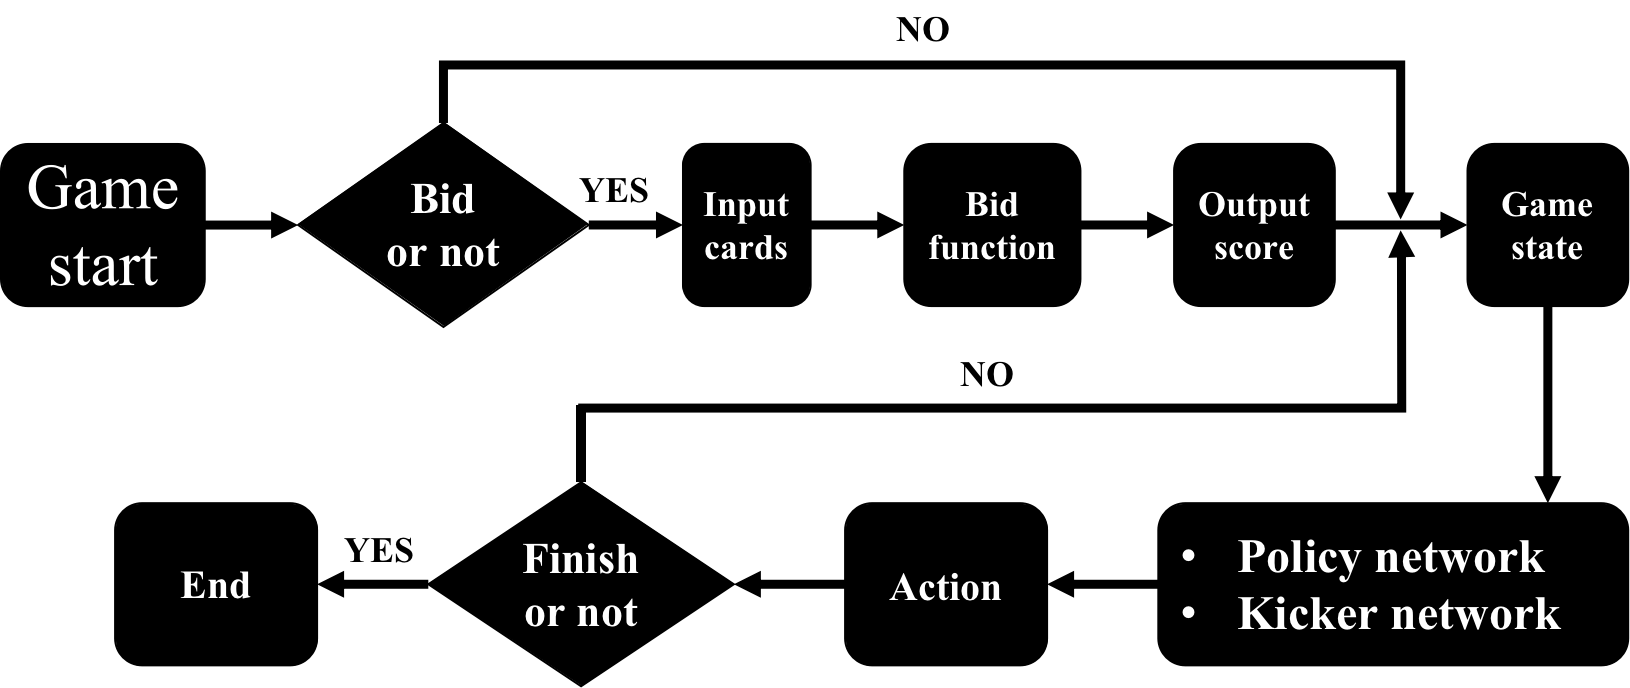
\includegraphics[width=10cm]{final_project_template/Images/gameflow.png}
    \label{gameflow} 
\end{figure}

\subsection{Related Work}
As so far, Libratus and DeepStack are the best AI programs in Texas Hold'em, they are developed by Carnegie Mellon University and University of Alberta respectively (\cite{brown2018superhuman},\cite{moravvcik2017deepstack}). We know Texas Hold'em is also imperfect information game, only DeepStack used deep neural network, but the problem is both of them can only be used in the one-to-one mode.

Many other Doudizhu AIs use different algorithm, some of them use Q-Learning or MCTS (\cite{you2019combinational}). We want to verify whether the model trained through CNN can achieve good results like them. 

\section{The Proposed Algorithm}

Our project can split into four parts. The first is Call Landlord Algorithm or we call it Bid Module. The second is generate game data using Minimax. Third is Policy net, which helps the player choose what cards to play. The Policy net is called before the AI will do action, the output of the Policy net may contain Kicker Card type (solo or pair) in some labels. Then here comes the forth part, Kicker net. If there is a Kicker card need to be predicted, the Kicker net is called.

\subsection{Call Landlord Algorithm}
In the reference paper\cite{liu2018solution}, we find that they do not design a strategy to judge to determine whether to bid. So we randomly generate 4048 sets of initial cards and marked them artificially. The label ``0'' represent ``Not Bid'' and the label ``1'' represent ``Bid''. Table \ref{Import} shows some data we generated and marked for Call Landlord Algorithm.

In statistics, the logistic model (or logic model)\cite{enwiki:1023179480} is used to model the probability of a certain class or event existing such as pass/fail, win/lose, alive/dead or healthy/sick. This can be extended to model several classes of events such as determining whether an image contains a cat, dog, lion, etc. Each object being detected in the image would be assigned a probability between 0 and 1, with a sum of one.

\begin{table}[!ht]
    \caption{Import dataset for Call Landlord Algorithm}\label{Import}
    \centering
    \begin{threeparttable}          
      \begin{tabular}{ccccccccccccccccc}\toprule
        Card & 3 & 4 & 5 & 6 & 7 & 8 &9 &10 &J &Q &K &A &2 &SJ &BJ &Bid\\ \hline
        Hand Card 1 &1 &1 &0 &2 &3 &2 &1 &3 &0 &0 &1 &2 &0 &1 &0 &0 \\ \hline
        Hand Card 2 &2 &1 &2 &2 &2 &1 &1 &1 &1 &0 &1 &1 &1 &0 &1 &1\\ \bottomrule
      \end{tabular}
         \begin{tablenotes}    
        \footnotesize               
        \item[1] ``Card'': The card from 3 to Big Joker.         
        \item[2] ``Hand Card'': The card you have after deal.
        \item[3] ``Bid'': Based on your Hand Card, bid or not.
      \end{tablenotes}          
    \end{threeparttable}  
  \end{table}

Because whether to bid is a binary classification problem, so we use Logistic Regression to decide it based on our Hand Card.

\subsection{Generate game data}
We want to train the model with the ``best'' data, so we assume that the player knows the cards of all other players and plays cards according to a certain strategy. Here we use Minimax algorithm to generate data.

\begin{table}[!ht]
    \caption{Card Scores}\label{CardScore}
    \centering
    \begin{threeparttable}          
      \begin{tabular}{cccccccccccccccc}\toprule
        Card & 3 & 4 & 5 & 6 & 7 & 8 &9 &10 &J &Q &K &A &2 &SJ &BJ \\ \hline
        Score &1 &2 &3 &4 &5 &6 &7 &8 &9 &10 &11 &12 &13 &14 &15 \\ \bottomrule
      \end{tabular}
    \end{threeparttable}  
  \end{table}
First, we set different scores for different cards, the scores are 1 to 15 from 3 to Big Joker(Table\ref{CardScore}). And the score for each node is calculate as:


$$
Score(Peasant) = \frac{Score (Peasant)}{num(Peasant \ remaining \ card)} $$
$$
Score(Landlord) = \frac{Score(Landlord)}{num(Landlord\  remaining \ card)}
$$

Then we construct a decision tree, in theory, we can get the global optimal solution by increasing the depth, but in real application, the depth of decision tree is very deep. It is really hard for us to find a global optimal decision. In this case, we searched 5 layer of the decision tree. 

In one game, we want to maximize the value of ``Landlord'' and minimize the value of ``Peasant'', as the value can be calculated as:

$$
Value = Score(Landlord)- \frac{Scoure(Peasant)}{2}
$$


Because of the hardware limitation, we generate 5,000 games and 194,078 samples. We upload our project to GitHubThe details of the program and dataset can be found in \url{https://github.com/Zzfiv3/doudizhu-rengongzhizhang}.

\subsection{Policy Net}
Policy Net is used to determine what type of cards to play. In this project, we built the Policy Net with 6 convolutional layer, 6 batch normolization layer and 1 full connection layer, use \textbf{ReLU} as activation function. A final softmax layer outputs probability distribution over all legal action $a$. The input represents current game state. The Policy Net is traine on randomly sampled state-action pairs ($s$,$a$). 

The input to the Policy Net is a 15$\times$20$\times$21 3-dimensional binary tensor. Each dimension along X-axis represents the ranks of cards, from 3 to Big Joker. Y-axis represents the number of each card (from 1 to 4), and features in Doudizhu, such as solo, pair, trio, etc. Z-axis represents the sequential information of each rounds, this design leaned from AlphaGo, make the variable length to fixed legth in game. In this project, we chose the most recent 6 rounds. $S_{i,j,k}$ standards the binary feature for current state of the game. Details are shown in Table\ref{Yinput} and Table \ref{Zinput}.

The Policy Net outputs 309 action probabilities after we add the Kicker Net to our module, see Table\ref{OutPolicy} for more details. It is noteworthy that the maximum number of cards is 20, it restricts the longest length of category.


Policy Net structure please see Figure \ref{PolicyNetFlow}.
\graphicspath{{Images/}}
\maketitle
\begin{figure}[htp]
    \caption{Policy Net structure} \label{PolicyNetFlow}
    \centering 
    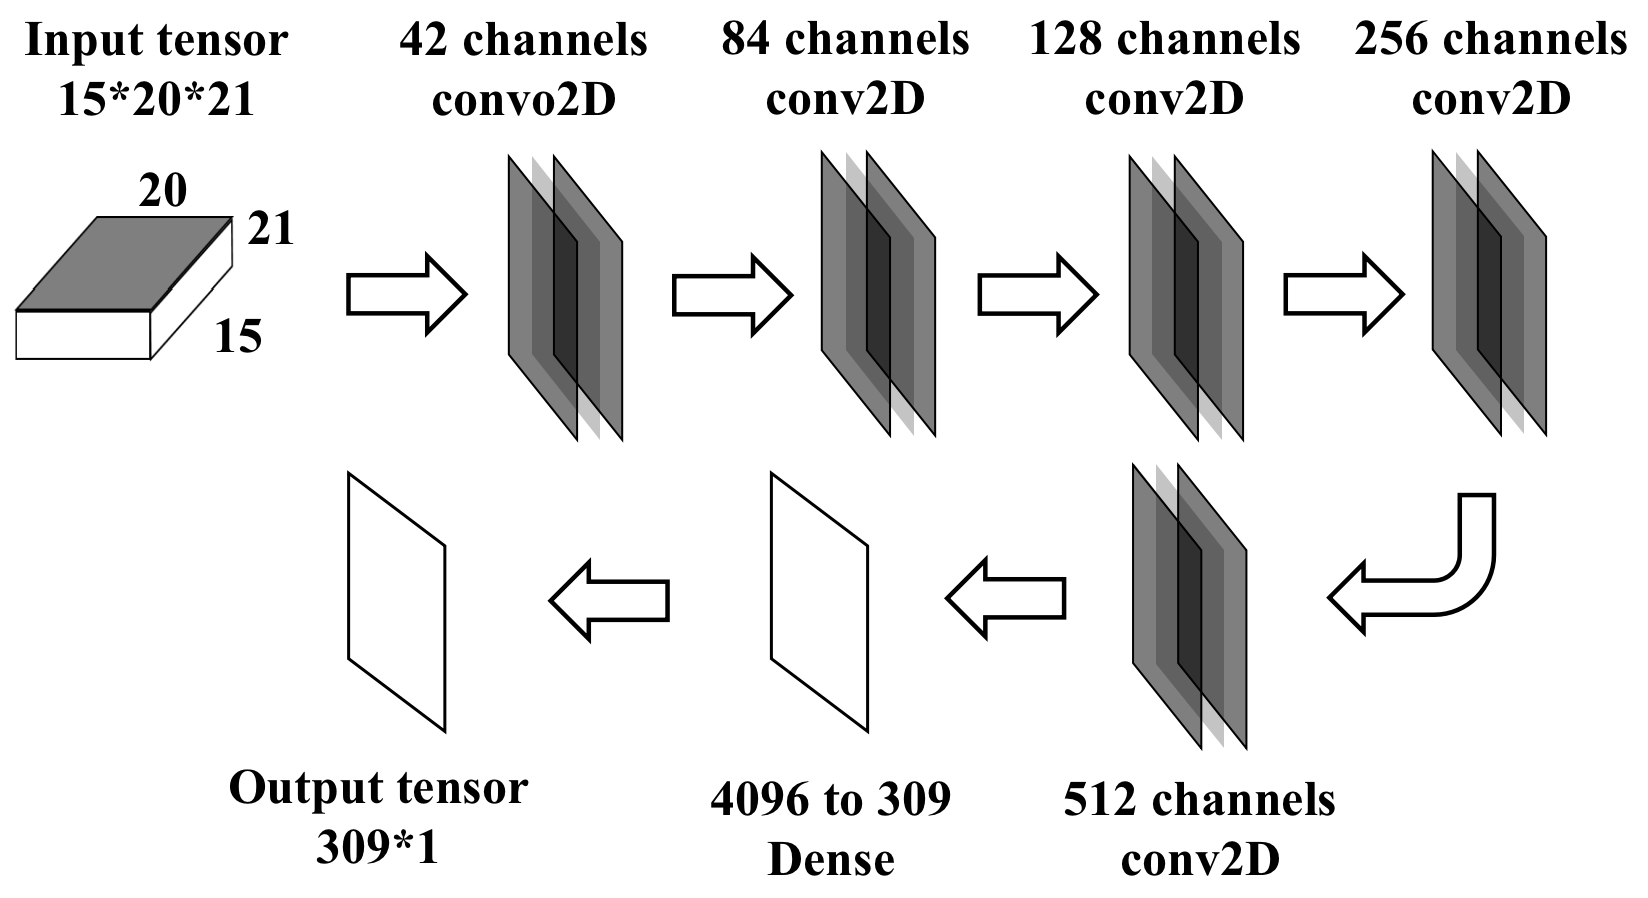
\includegraphics[width=10cm]{PolicyNet1}
    \label{PolicyNetFlow} 
\end{figure}

\subsection{The Kicker Net}

After judging whether to call landlord in Bid Module and choosing card policies in Policy Net, we can play a game in principle. Nevertheless, there is still a problem to judge the kicker cards. If there are $n$ choices for the Main Group decided by the Policy Net and $m$ choices for the Kicker Cards, then there exists $n \times m$ available actions in total. In some other cases, if the player has trio with chain (e.g.  \textbf{\textit{555666}} is a trio with chain), the length is \textbf{\textit{i}} (the length of \textbf{\textit{555666}} is 2), and \textbf{\textit{j}} for available Kicker Cards, then there exists $C_j^i$ choice in total.

In order to address this problem, we add a Kicker Net after the Policy Net. The Policy Net predict the Main Group cards and type of the Kicker Cards. The Kicker type includes triplet with an attached card, triplet with an attached pair, sequence of triplets with attached cards and sequence of triplets with attached pairs. 

The input of the Kicker Net is a 15$\times$8$\times$1 3-dimensional binary tensor. Each dimension along \textit{X-axis} represents the cards type, from \textbf{\textit{3}} to \textbf{\textit{Big Joker}}. The first four dimensions of \textit{Y-axis} includes the kicker-cards type information, and the last four dimensions includes the remaining handcards information. The output of the Kicker Net is a 28$\times$1 2-dimension probability values of each kicker card, include fifteen kinds of solo and thirteen kinds of pairs. The input of Kicer Net please see Table \ref{YoutKicker}. And the structure of Kicker Net please see Figure\ref{kicernetnew}. 

\graphicspath{{Images/}}
\maketitle
\begin{figure}[htp]
    \caption{Kicker Net structure} \label{kicernetnew}
    \centering 
    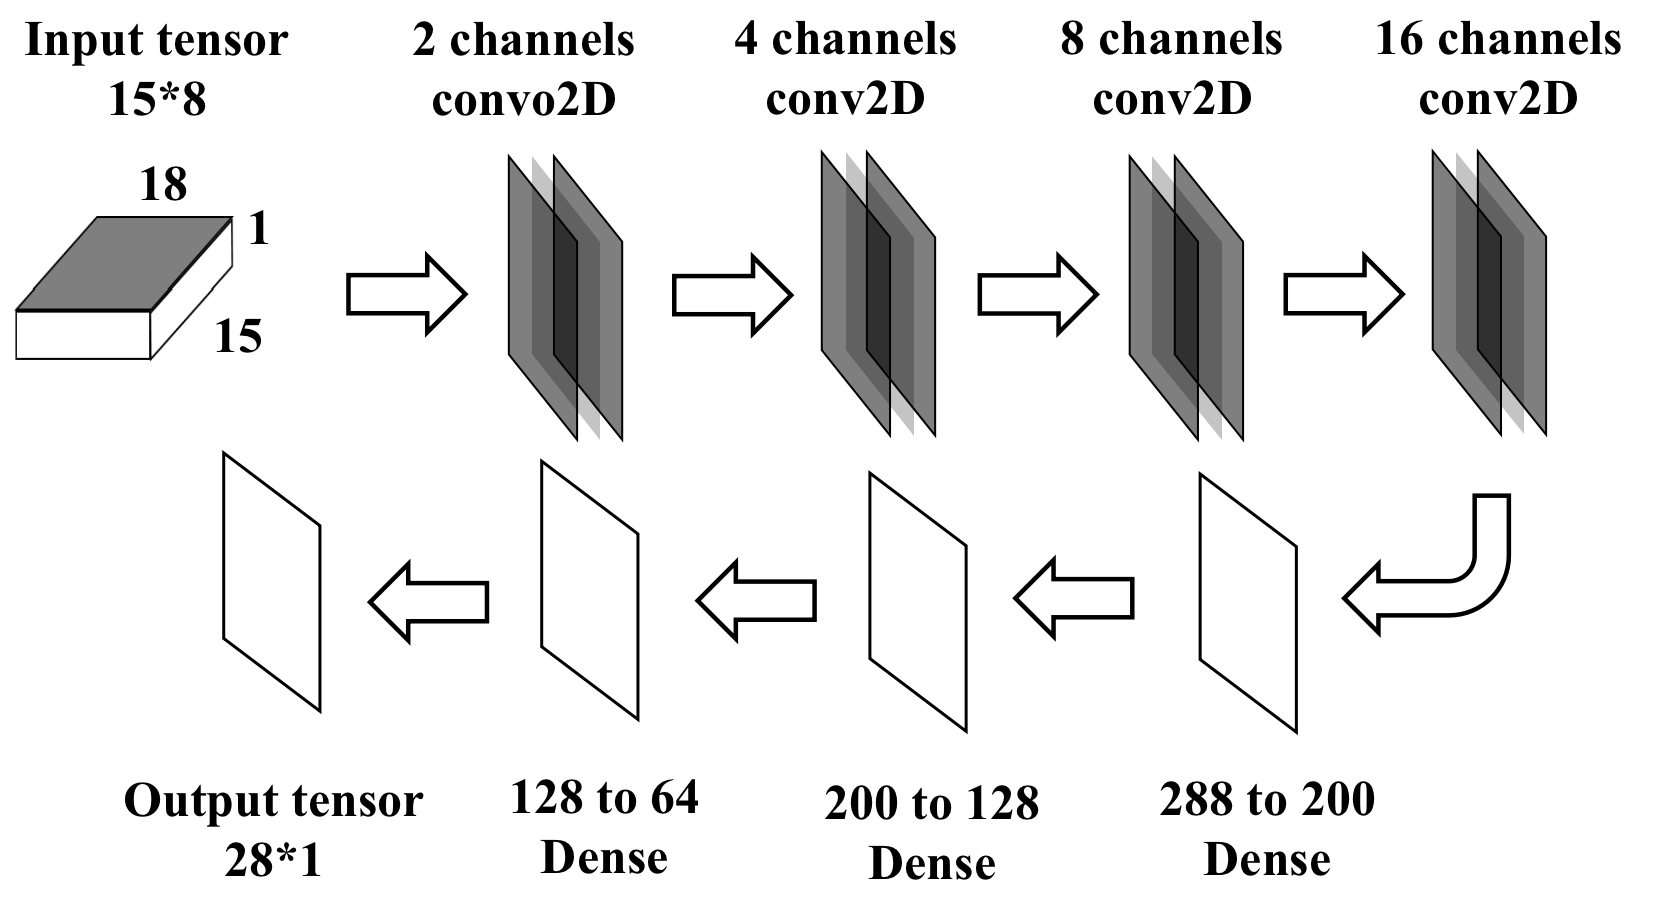
\includegraphics[width=10cm]{final_project_template/Images/KickerNetNew2.png}
\end{figure}

In this network, we use four convolution layers, four batch-normalization layers after each convolution layer and three full-connection layers. We choose \textbf{ReLU} as the activation function after each convolution layer and choose Softmax after the full-connection layer in order to obtain the probability of each kicker card. The Kicker Net choose the max-probability type as the output cards.

% Please add the following required packages to your document preamble:
% \usepackage[table,xcdraw]{xcolor}
% If you use beamer only pass "xcolor=table" option, i.e. \documentclass[xcolor=table]{beamer}


The experiment should first state the dataset overview, evaluation metric and implementation details; then a sub-section on individual component analysis should be followed (why component A is necessary in my algorithm; what if A is removed, or A is replaced with B); the last part should list the performance comparison between the proposed method and previous state-of-the-arts.

Since we have a tight paper length requirement, you can put some parts of the experiments in the Appendix section if your paper is over-length.

\section{Experiments}
\subsection{Call Landlord Experiment}
 We use 3036 data to train and use 1012 data to test. The accuracy is 93.3$\%$. By observing the coefficient matrix \ref{clcoef}, we can find that bid or not mainly based on the number of card 2, Small Joker and Big Joker.
 
\graphicspath{{Images/}}
\maketitle
\begin{figure}[htp]
    \caption{Call Landlord Coefficient} \label{clcoef}
    \centering 
    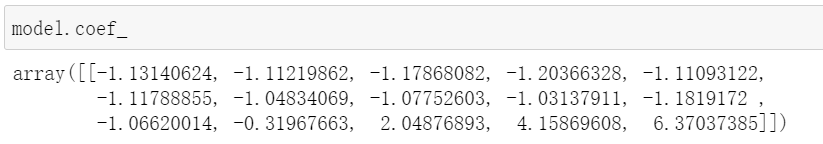
\includegraphics[width=12cm]{final_project_template/Images/clcoef.png}
\end{figure}

\subsection{Policy Net Experiment}

We used 5,000 game records for training the Policy Net. One record represent a complete game, and can be divided into many state-action pairs, from several rounds to more than twenty rounds, depending on length of the records. After divide all game records, we get 194,078 state samples. The accuracy and the loss of the model are shown in Figure \ref{policyAcc}.
\graphicspath{{Images/}}
\maketitle
\begin{figure}[htp]
    \caption{Accuracy and Loss of Policy Net} \label{policyAcc}
    \centering 
    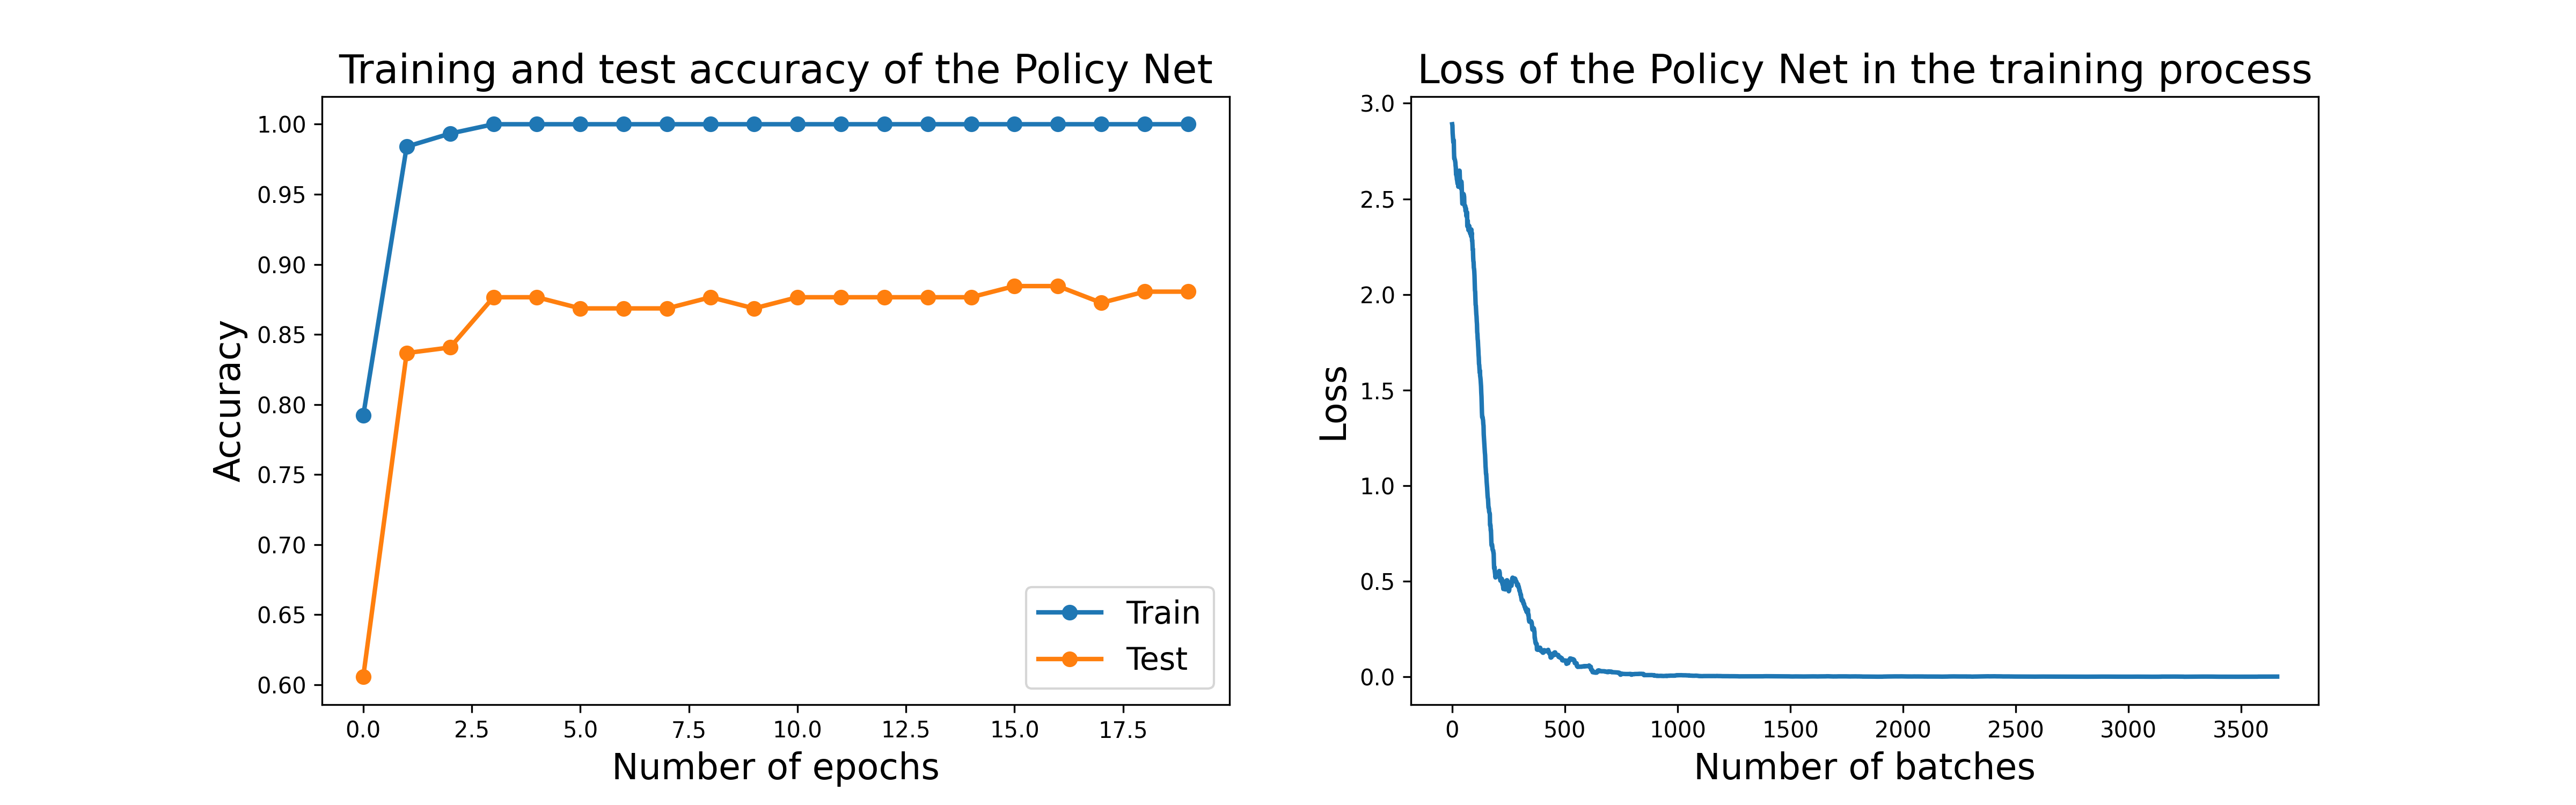
\includegraphics[width=15cm]{final_project_template/Images/policyAcc.png}
\end{figure}

\subsection{Kicker Net}

We used 9,242 samples for training the Kicker Net. Train the data for 20 epochs, the accuracy and the loss are shown in Figure \ref{kickerAcc}

\graphicspath{{Images/}}
\maketitle
\begin{figure}[htp]
    \caption{Accuracy and Loss of Kicker Net} \label{kickerAcc}
    \centering 
    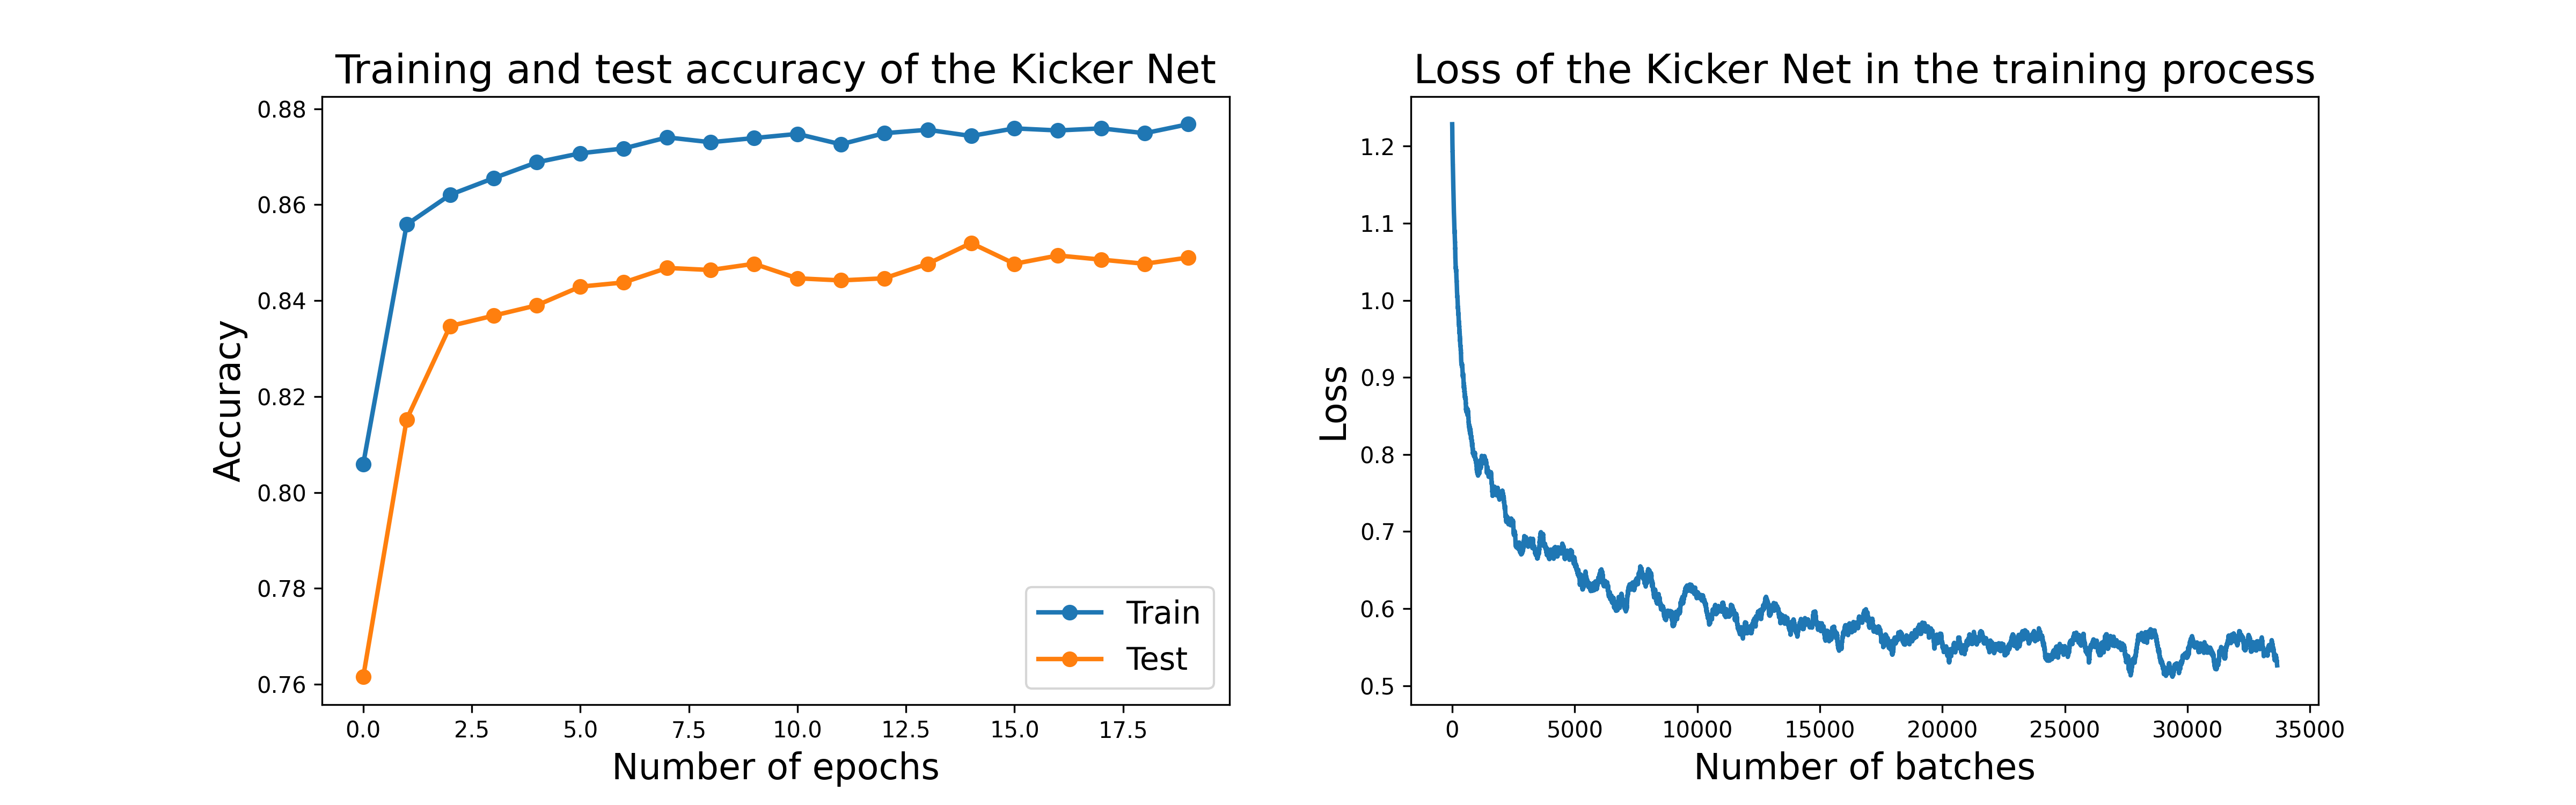
\includegraphics[width=15cm]{final_project_template/Images/Acc.png}
\end{figure}

\section{Discussions}

1.From the training data of the Policy Net and Kicker Net, we find these two models are able to complete some simple prediction based on the remaining handcards and the recorded round information.

2.Our model is built based on our subjective consciousness, like the design of Minimax Algorithm, and the Z-axis of Policy Net. Maybe there are better ways to design the model.

3.Also, because of the hardware limitation, we can only generate 5,000 game records. If we get more time to optimize our program, we believe we can get more dataset and get a better performance.

4.About the Call Landlord Algorithm, we marked the label by ourselves, which makes the labels very subjective. Because we don’t know if others will adopt different strategies for the same deck of cards.


\bibliographystyle{ieee}
\bibliography{dl}



\clearpage
\section*{Appendix}

\begin{table}[!ht]
    \caption{Meaning of each plane (Y-axis) of the input matrix}\label{Yinput}
    \centering
    \begin{threeparttable}          
      \begin{tabular}{cc}\toprule
Dimensions & Meaning                         \\ \hline
0          & Pass                            \\
1          & Solo                            \\
2          & Solo chain                      \\
3          & Pair                            \\
4          & Pair chain                      \\
5          & Trio                            \\
6          & Trio chain                      \\
7          & Bomb/Rocket                     \\
8          & Trio with solo kicker           \\
9          & Trio with pair kicker           \\
10         & Four with solo kickers          \\
11         & Four with pair kickers          \\
12         & Plane with solo kickers         \\
13         & Plane with pair kickers         \\
14         & Number of rounds                \\
15         & Number remaining of each player \\
16         & Number of remaining cards (1)   \\
17         & Number of remaining cards (2)   \\
18         & Number of remaining cards (3)   \\
19         & Number of remaining cards (4)  \\ \hline
      \end{tabular}
    \end{threeparttable}  
  \end{table}
  
\begin{table}[!ht]
    \caption{Meaning of each plane (Z-axis) of the input matrix}\label{Zinput}
    \centering
    \begin{threeparttable}          
      \begin{tabular}{cc}\toprule
        
Planes & Meaning                                        \\ \hline
1      & All cards played out before last 6 rounds.     \\
2-4    & The cards played out in the sixth last round.  \\
5-7    & The cards played out in the fifth last round.  \\
8-10   & The cards played out in the fourth last round. \\
11-13  & The cards played out in the third last round.  \\
14-16  & The cards played out in the second last round. \\
17-19  & The cards played out in the most recent round. \\
20     & All cards has that have not been seen yet      \\
21     & All cards in hand                              \\ \hline
      \end{tabular}
    \end{threeparttable}  
  \end{table}
  
  
\begin{table}[!ht]
    \caption{Output of the Policy Net}\label{OutPolicy}
    \centering
    \begin{threeparttable}          
      \begin{tabular}{cc}\toprule
        
Primal type             & Number of possibilities \\ \hline
Solo                    & 15                      \\
Solo chain              & 36                      \\
Pair                    & 13                      \\
Pair chain              & 52                      \\
Trio                    & 13                      \\
Trio chain              & 45                      \\
Trio with solo kicker   & 13                      \\
Plane with solo kickers & 38                      \\
Trio with pair kicker   & 13                      \\
Plane with pair kickers & 30                      \\
Four with solo kickers  & 13                      \\
Four with pair kickers  & 13                      \\
Bomb                    & 13                      \\
Rocket                  & 1                       \\
Pass                    & 1                       \\ \hline
sum                     & 309                     \\ \hline
      \end{tabular}
    \end{threeparttable}  
  \end{table}

\begin{table}[!ht]
    \caption{Meaning of Y-axis of the input of Kicker Net}\label{YoutKicker}
    \centering
    \begin{threeparttable}          
      \begin{tabular}{cc}\toprule
        
Dimension & Meaning                       \\ \hline
0         & Trio with solo kicker         \\
1         & Trio with pair kicker         \\
2         & Four with solo kickers        \\
3         & Four with pair kickers        \\
4         & Number of remaining cards (1) \\
5         & Number of remaining cards (2) \\
6         & Number of remaining cards (3) \\
7         & Number of remaining cards (4) \\ \hline
      \end{tabular}
    \end{threeparttable}  
  \end{table}



\end{document}

